\emph{This chapter gives a general overview of hydraulic systems and an introduction to the WSS in Randers. The typical topologies and components of drinking water supply networks are discussed. The specific distribution zones, pumping stations, waterworks and WTs are introduced and their detailed operation is explained in the Randers WSS.}

\section{Hydraulic systems overview}
\label{hydraulic_system_overview}

WSSs are designed to deliver water to consumers in terms of sufficient pressure and appropriate chemical composition, while a safe and efficient operation is satisfied at all time. Drinking water distribution systems need to transport water from one geographical place to another. In practice, several different methods exist to achieve such water transport. One example is to use the natural advantages such as the water stored in mountains, and thereby use the potential energy of the water to provide pressure in the supply area. A good example for this are countries like Norway where the advantages of the landscape can be utilized \cite{norway_mountains}. However, considering the fact that in Denmark typically water is tapped from the ground, such advantages cannot be taken into account, unless the water is first pumped to high elevation points. Furthermore, it is worth noting that the quality of groundwater, in general, is very good in Denmark and therefore primarily used for drinking water purposes. In some areas, the water is clean enough to go through only an aeration process at the waterworks, right after tapping it from the ground. 

In WSSs, the two main actuators are pumps and valves. These two kind of control elements make it possible to pump the clean water into the network and thereby to deliver the water to the costumers or to WTs, where the water can be stored for later use \cite{prahata}. The schematic of the water delivery process is illustrated in \figref{fig:WSS_example}.

%illustration of WSS
\begin{figure}[H]
\centering
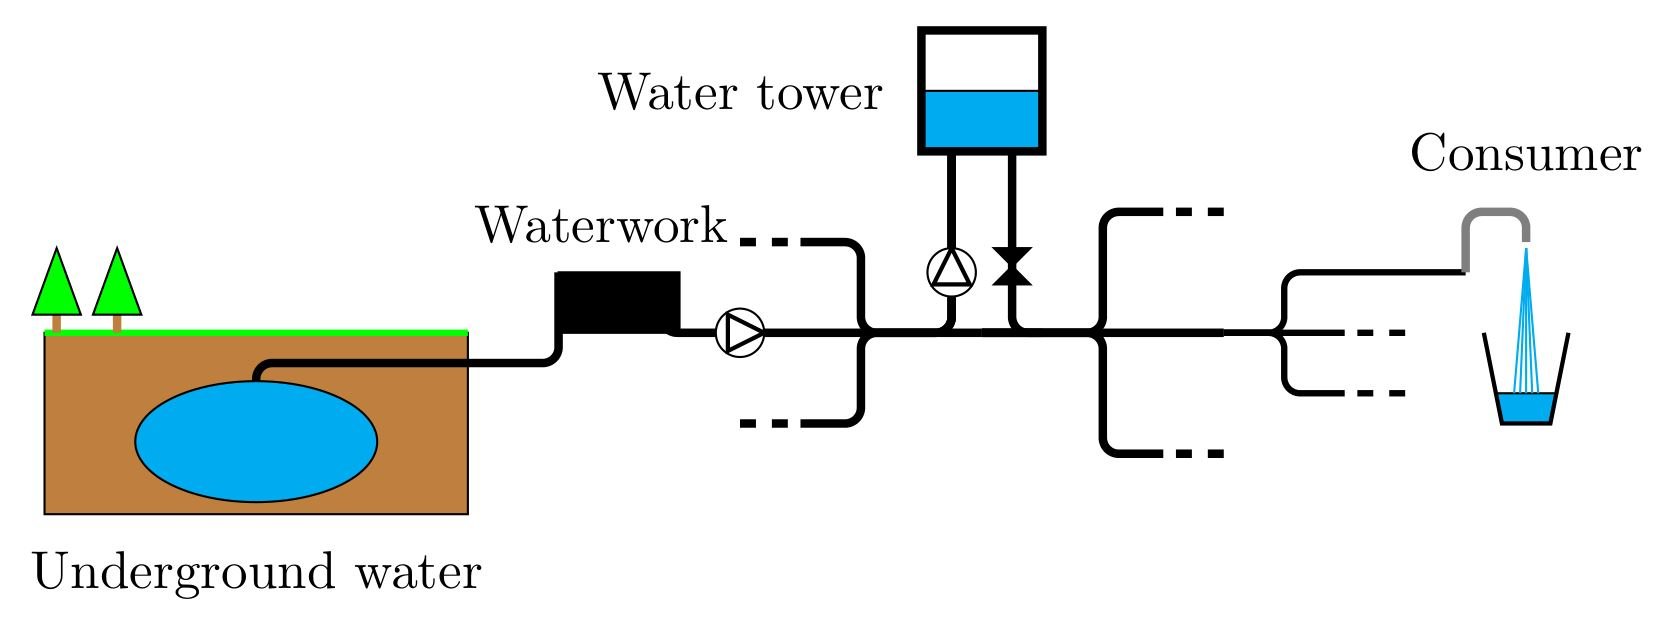
\includegraphics[width=0.63\textwidth]{report/pictures/WSS_illustration}
\caption{Illustration of a WSS \cite{kenneth_houe}.}
\label{fig:WSS_example}
\end{figure}

\vspace{-3mm}

Additionally, the delivered water needs to fulfil certain pressure criteria in order to reach consumers at higher levels. For example, in some cases the pressure has to be high enough to make it to the fourth floor of a building and still provide appropriate pressure in the water taps. Generally, in such cases booster pumps are placed in the basement of the building, helping the supply. In case of high geographical locations, water is typically stored in WTs, thereby allowing to take advantage of the potential energy of the water. Additionally to the case of low pressure, it should be noted that too high pressure increases water losses due to pipe waste, e.g. leakages \cite{walski2003advanced}.

Another criteria is that the flow through particular pipes need to stay within acceptable limits. A low flow rate can lead to water quality problems due to the undesirable micro organisms in the water and due to the metal and salt accumulation on the wall of the pipes \cite{walski2003advanced}. 

As it is shown in \figref{fig:WSS_example}, typically WSSs consist of pipe, valve, reservoir, WTs and pump components. The common property of them is that they are all two-terminal components, therefore they can be characterized by the relation between the pressure drop across their two corresponding endpoints and the flow through them \cite{master_aau}. 

\subsection{Pipe networks}
\label{pipe_networks}

Pipes have a major role in WSSs since they are used for carrying pressurized water. They serve as a connection between components. Normally, the network can be split into different sub-parts, taking into account the physical characteristics and the attributes of the pipes. Therefore, water supply networks can consist of transmission mains, arterial mains, distribution mains and service lines as shown in \figref{fig:pipemain_example}.

%illustration of pipe topology / loop configuration
\begin{figure}[H]
\centering
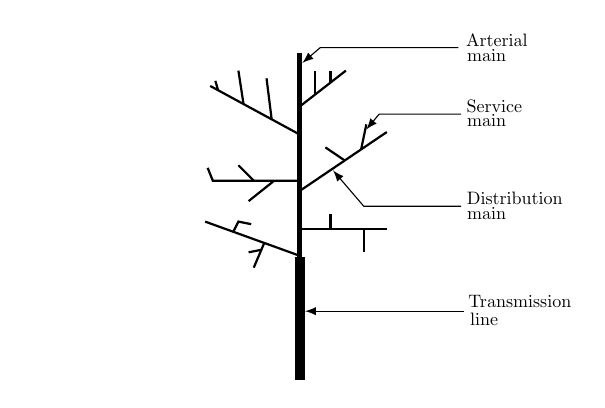
\begin{tikzpicture}[scale=0.65,transform shape]

\fill [black] (0.1,0.1) rectangle (0.3,2.5);
\fill [black] (0.15,6.5) rectangle (0.25,2.5);

\draw [thick](0.15,2.55) -- (-1.65,3.2);
\draw [thick](-0.5,2.77) -- (-0.7,2.3);
\draw [thick](-0.55,2.65) -- (-0.8,2.6);
\draw [thick](-1.1,3) -- (-1,3.2) -- (-0.75,3.15);
\draw [thick](0.2,3.05) -- (1.9,3.05);
\draw [thick](0.8,3.05) -- (0.8,3.35);
\draw [thick](1.45,3.05) -- (1.45,2.6);
\draw [thick](0.2,4) -- (-1.5,4) -- (-1.6,4.25);
\draw [thick](-0.3,4) node (v1) {} -- (-0.8,3.6);
\draw [thick](v1);
\draw [thick](-0.7,4) -- (-1,4.3);
\draw [thick](0.2,3.8) -- (1.9,4.95);
\draw [thick](1.4,4.62) -- (1.5,5.1);
\draw [thick](1.07,4.4) -- (0.7,4.65);
\draw [thick](0.2,4.9) -- (-1.55,5.85);
\draw [thick](-0.35,5.2) -- (-0.45,6);
\draw [thick](-0.9,5.5) -- (-1,6.15);
\draw [thick](-1.4,5.78) -- (-1.45,5.95);
\draw [thick](0.2,5.45) -- (1.1,6.15);
\draw [thick](0.8,5.92) -- (0.8,6.15);
\draw [thick](0.5,5.69) -- (0.5,6.15);
%\draw [-latex](3.4,1.45) -- (0.3,1.85);
\node at (4.5,1.65) {\normalsize Transmission};
\node at (3.8,1.3) {\normalsize line};
%\draw [-latex](3.35,3.4) -- (0.6,4.05);
\node at (4.4,3.65) {\normalsize Distribution};
\node at (3.85,3.35) {\normalsize main};
\node at (4,5.45) {\normalsize Service};
\node at (3.85,5.17) {\normalsize main};
\node at (4.05,6.75) {\normalsize Arterial};
\node at (3.85,6.45) {\normalsize main};
%\draw [-latex](3.25,5.25) -- (1.5,5);
%\draw [-latex](3.2,6.55) -- (0.25,6.4);
\node at (-5,3.6) {         };
\draw [-latex](3.3,6.6) -- (0.6,6.6) -- (0.25,6.3);
\draw [-latex](3.35,5.3) -- (1.75,5.3) -- (1.5,5);
\draw [-latex](3.35,3.5) -- (1.45,3.5) -- (0.85,4.2);
\draw [-latex](3.4,1.45) -- (0.3,1.45);
\end{tikzpicture} 
\caption{Illustration of pipe mains. Tree configuration.}
\label{fig:pipemain_example}
\end{figure}

\vspace{-3mm}

Transmission mains deliver large amounts of water over long distances. Arterial and distribution mains provide intermediate steps towards delivering water to the end-users. Service lines transmit the water from the distribution mains straight to the end-users \cite{grigg2012water}.

The transmission and distribution network can have a topology that is called a loop or a tree structure. \figref{fig:pipemain_example} shows an example for a tree configuration. This type of configuration is most frequently used in rural areas \cite{mays}. Typically the network has only one path for the water to reach the end-users. A more frequent problem compared to looped configurations is, that on the outer parts of the system lower pressures can be experienced due to the pressure losses from long flow paths. The flow dynamics within this kind of systems therefore consist of large flows closer to the source that turn into smaller flows on the outer parts of the system. Main disadvantage of a purely tree structure system is that due to maintenance or momentary breakdowns, the system suffers disruption of service \cite{mays}. 

Loop networks have a configuration as shown in \figref{fig:loop_configuration}. 

%illustration of loop configuration
\begin{figure}[H]
\centering
 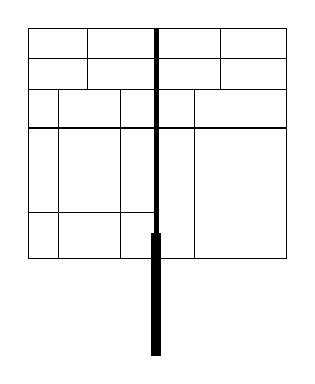
\begin{tikzpicture}[scale=0.65,transform shape]
 
 
\fill [black] (0.1,0.1) rectangle (0.3,2.5);
\fill [black] (0.15,6.5) rectangle (0.25,2.5);


%\node at (-6,3.6) {         };

\draw (0.2,6.5) -- (2.75,6.5) -- (2.75,2) -- (0.3,2);
\draw (0.2,6.5) -- (-2.3,6.5) -- (-2.3,2) -- (0.1,2);
\draw (-2.3,5.3) -- (2.75,5.3);
\draw (-2.3,5.9) -- (2.75,5.9);
\draw (-1.15,6.5) -- (-1.15,5.3);
\draw (1.45,6.5) -- (1.45,5.3);
\draw (-1.7,5.3) -- (-1.7,2);
\draw (-0.5,5.3) -- (-0.5,2);
\draw (-2.3,4.55) -- (0.15,4.55);
\draw (-2.3,2.9) -- (0.15,2.9);
\draw (0.95,5.3) -- (0.95,2);
\draw (0.2,4.55) -- (2.75,4.55);
\end{tikzpicture} 
%
\includegraphics[width=0.35\textwidth]{report/pictures/missingfigure}
\caption{Loop configuration.}
\label{fig:loop_configuration}
\end{figure}

\vspace{-3mm}

Loop networks are usually composed of smaller loops which are composed of smaller distribution mains, and larger loops that are connected to arterial or transmission mains. WTs are typically placed in the center of the system due to pressure losses resulting from flows through the loop network \cite{council2007drinking}. This is reasonable because within a certain grid, the same pressure is provided by the tank, instead of providing the pressure through long pipelines to different distances. Furthermore, in the presence of a ring structure, the large loop around the area may be used to feed an internal distribution grid or a distribution grid attached to the outer part of the loop. Loop configurations are generally associated with larger suburban and city distribution systems such as larger cities\cite{council2007drinking}. It is worth mentioning that certain parts of the WSS in Randers fall into both categories. Similarly as in the Randers WSS, the pipelines in the outer parts or in newly connected parts have tree structures. Grid structure is more typical in the city center of big cities. 

\subsection{Elevated reservoirs}
\label{elevated_reservoirs}

Elevated reservoirs, or equivalently WTs, are typically present in the system in order to use them as buffers and level out the pressure and flow demand differences. When the demand is high, the waterworks might not be able to provide the sufficient amount of water in the network. In this case, the WT supplies the remaining demand. When the user consumption decreases, the system can be controlled such that the WT is being refilled to provide the required demand for the next peak time of the consumption. Having WTs in the network, the system becomes more independent from the pumping stations, meaning that the refilled tank can itself maintain the desired pressure and flow for a limited time. 

Due to the elevation of the tank, when it is filled up, the pumping stations need to provide a pressure higher than the pressure in the WT. Therefore when the tank is being emptied, the pumping stations can reduce the amount of pressure they provide to the system, since the pressure from the elevated reservoir becomes dominant. This is due to the fact that the dynamics of WSSs with large storages come primarily from the pressure of the WTs \cite{8thsemester_project}. However, it should be noted that normally the level in the tank is varying less than a meter. This means that the effect on the pump operation is limited. Due to these considerations, the dynamics of WTs has to be taken into account while modelling a WSS. 

\subsection{Pumps}
\label{pumps}

Water pumps are used to increase pressure in hydraulic systems, thus making the water flow. Pumps are typically the main actuators of a WSS and they can be either flow or pressure controlled. The control is done by changing the rotational speed of the pump. Therefore, the pump has a reference and simple control makes it possible to produce the desired flow and pressure \cite{kallesoePHD}.The pressure required to make the water reach some height is the sum of the pressure required to overcome the elevation and the friction losses in the pipe network. 

In WSSs, typically centrifugal pumps are used. The characteristics of such pumps are described by two pump curves. The two curves depict the volume flow versus the pressure and the power of the pump, respectively. Normally the curves describe the characteristics for one particular speed, which is the nominal speed \cite{kallesoePHD}. An example of the two pump curves is shown in \figref{fig:pump_curves}.

\begin{figure}[H]
\centering
\begin{subfigure}{.49\textwidth}
\centering
  % This file was created by matlab2tikz.
%
%The latest updates can be retrieved from
%  http://www.mathworks.com/matlabcentral/fileexchange/22022-matlab2tikz-matlab2tikz
%where you can also make suggestions and rate matlab2tikz.
%
\definecolor{mycolor1}{rgb}{0.00000,0.44700,0.74100}%
%
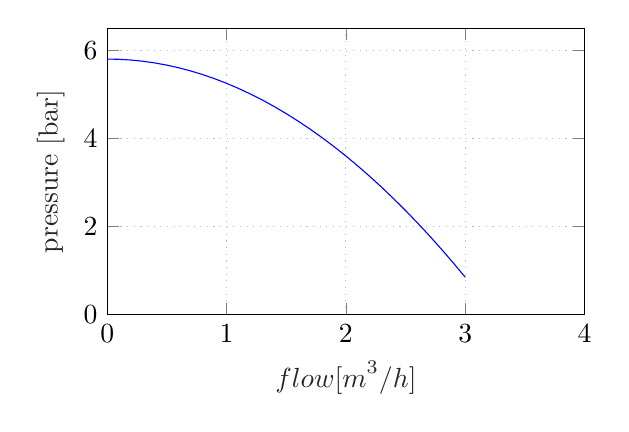
\begin{tikzpicture}

\begin{axis}[%
width=0.5\textwidth,
height=0.3\textwidth,
at={(0.758in,0.499in)},
scale only axis,
xmin=0,
xmax=4,
xlabel style={font=\color{white!15!black}},
xlabel={$\text{flow [m}^\text{3}\text{/h]}$},
ymin=0,
ymax=6.5,
ylabel style={font=\color{white!15!black}},
ylabel={pressure [bar]},
axis background/.style={fill=white},
xmajorgrids,
ymajorgrids,
grid style={dotted}
]
\addplot [color=blue, forget plot]
  table[row sep=crcr]{%
0	5.8\\
0.0999999999999996	5.7945\\
0.2	5.778\\
0.3	5.7505\\
0.4	5.712\\
0.5	5.6625\\
0.600000000000001	5.602\\
0.7	5.5305\\
0.8	5.448\\
0.9	5.3545\\
1	5.25\\
1.1	5.1345\\
1.2	5.008\\
1.3	4.8705\\
1.4	4.722\\
1.5	4.5625\\
1.6	4.392\\
1.7	4.2105\\
1.8	4.018\\
1.9	3.8145\\
2	3.6\\
2.1	3.3745\\
2.2	3.138\\
2.3	2.8905\\
2.4	2.632\\
2.5	2.3625\\
2.6	2.082\\
2.7	1.7905\\
2.8	1.488\\
2.9	1.1745\\
3	0.85\\
};
\end{axis}
\end{tikzpicture}% 
  \caption{Flow versus pressure difference}
  \label{fig:sub1}
\end{subfigure}
\begin{subfigure}{.49\textwidth}
\centering
\vspace{-0.4mm}
% This file was created by matlab2tikz.
%
%The latest updates can be retrieved from
%  http://www.mathworks.com/matlabcentral/fileexchange/22022-matlab2tikz-matlab2tikz
%where you can also make suggestions and rate matlab2tikz.
%
\definecolor{mycolor1}{rgb}{0.00000,0.44700,0.74100}%
%
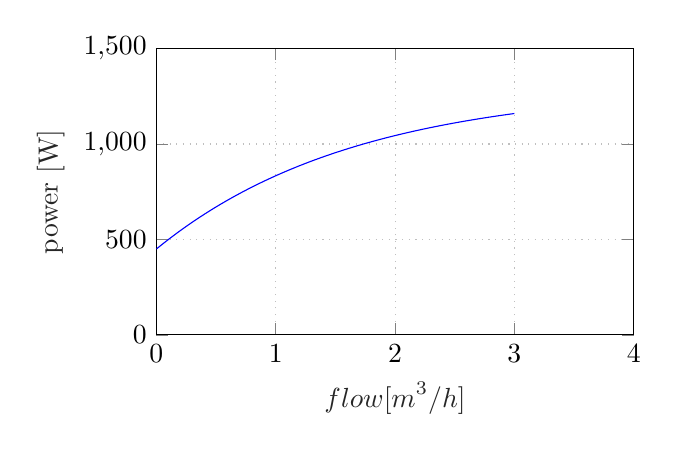
\begin{tikzpicture}

\begin{axis}[%
width=0.5\textwidth,
height=0.3\textwidth,
at={(0.758in,0.499in)},
scale only axis,
xmin=0,
xmax=4,
xlabel style={font=\color{white!15!black}},
xlabel={$\text{flow [m}^\text{3}\text{/h]}$},
ymin=0,
ymax=1500,
ylabel style={font=\color{white!15!black}},
ylabel={power [W]},
axis background/.style={fill=white},
xmajorgrids,
ymajorgrids,
grid style={dotted}
]
\addplot [color=blue, forget plot]
  table[row sep=crcr]{%
0	450\\
0.0599999999999454	480.055750539345\\
0.119999999999891	509.048738560475\\
0.180000000000064	537.01654303413\\
0.240000000000009	563.995414149676\\
0.299999999999955	590.020320300419\\
0.3599999999999	615.124993407542\\
0.420000000000073	639.341972641396\\
0.480000000000018	662.702646596815\\
0.539999999999964	685.237293977134\\
0.599999999999909	706.975122839624\\
0.660000000000082	727.944308453222\\
0.720000000000027	748.172029817625\\
0.779999999999973	767.684504891077\\
0.839999999999918	786.507024572515\\
0.900000000000091	804.663985482109\\
0.960000000000036	822.178921582701\\
1.01999999999998	839.074534683114\\
1.07999999999993	855.372723862874\\
1.1400000000001	871.094613856482\\
1.20000000000005	886.260582434024\\
1.25999999999999	900.890286813621\\
1.31999999999994	915.002689139926\\
1.38000000000011	928.616081061725\\
1.44000000000005	941.74810744047\\
1.5	954.415789220491\\
1.55999999999995	966.635545490521\\
1.61999999999989	978.423214765135\\
1.68000000000006	989.79407551368\\
1.74000000000001	1000.76286596331\\
1.79999999999995	1011.3438032018\\
1.8599999999999	1021.55060160486\\
1.92000000000007	1031.39649061192\\
1.98000000000002	1040.89423187328\\
2.03999999999996	1050.05613579107\\
2.09999999999991	1058.8940774752\\
2.16000000000008	1067.41951213515\\
2.22000000000003	1075.64348992761\\
2.27999999999997	1083.57667027892\\
2.33999999999992	1091.22933570126\\
2.40000000000009	1098.6114051202\\
2.46000000000004	1105.73244673099\\
2.51999999999998	1112.60169040034\\
2.57999999999993	1119.22803962954\\
2.6400000000001	1125.62008309472\\
2.70000000000005	1131.78610577893\\
2.75999999999999	1137.73409971065\\
2.81999999999994	1143.47177432257\\
2.88000000000011	1149.00656644414\\
2.94000000000005	1154.34564994065\\
3	1159.49594501165\\
};
\end{axis}
\end{tikzpicture}% 
\vspace{0mm}
  \caption{Flow versus power consumption}
  \label{fig:sub2}
\end{subfigure}
\caption{Pump curves describing the performance of a centrifugal pump at nominal speed.}
\label{fig:pump_curves}
\end{figure}

% %pump curves
% \begin{figure}[H]
% \centering
% % This file was created by matlab2tikz.
%
%The latest updates can be retrieved from
%  http://www.mathworks.com/matlabcentral/fileexchange/22022-matlab2tikz-matlab2tikz
%where you can also make suggestions and rate matlab2tikz.
%
\definecolor{mycolor1}{rgb}{0.00000,0.44700,0.74100}%
%
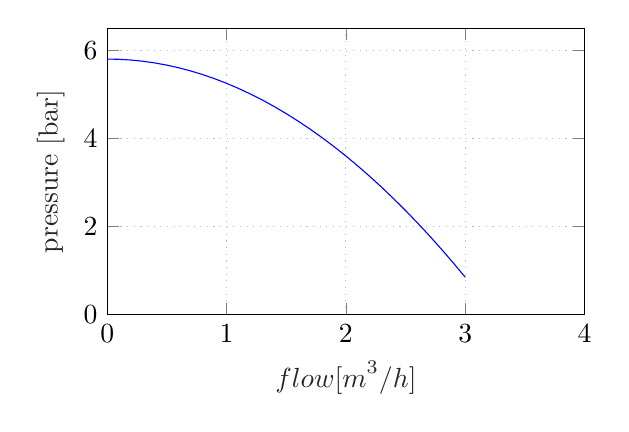
\begin{tikzpicture}

\begin{axis}[%
width=0.5\textwidth,
height=0.3\textwidth,
at={(0.758in,0.499in)},
scale only axis,
xmin=0,
xmax=4,
xlabel style={font=\color{white!15!black}},
xlabel={$\text{flow [m}^\text{3}\text{/h]}$},
ymin=0,
ymax=6.5,
ylabel style={font=\color{white!15!black}},
ylabel={pressure [bar]},
axis background/.style={fill=white},
xmajorgrids,
ymajorgrids,
grid style={dotted}
]
\addplot [color=blue, forget plot]
  table[row sep=crcr]{%
0	5.8\\
0.0999999999999996	5.7945\\
0.2	5.778\\
0.3	5.7505\\
0.4	5.712\\
0.5	5.6625\\
0.600000000000001	5.602\\
0.7	5.5305\\
0.8	5.448\\
0.9	5.3545\\
1	5.25\\
1.1	5.1345\\
1.2	5.008\\
1.3	4.8705\\
1.4	4.722\\
1.5	4.5625\\
1.6	4.392\\
1.7	4.2105\\
1.8	4.018\\
1.9	3.8145\\
2	3.6\\
2.1	3.3745\\
2.2	3.138\\
2.3	2.8905\\
2.4	2.632\\
2.5	2.3625\\
2.6	2.082\\
2.7	1.7905\\
2.8	1.488\\
2.9	1.1745\\
3	0.85\\
};
\end{axis}
\end{tikzpicture}% 
% %
\includegraphics[width=0.35\textwidth]{report/pictures/missingfigure}
% \caption{Loop configuration.}
% \label{fig:pump curves}
% \end{figure}

\vspace{-3mm}

As can be seen, at a given flow, the pump can deliver a pressure with a maximum limit. This pressure decreases when the flow is increasing. At a certain flow and pressure value, the pump has an optimal point where the operation is the most energy efficient. Pumps are normally designed such that the optimal point lies in the operational area for the pumping application \cite{kenneth_houe}. 

In some cases the required operating conditions for a WSS are beyond the reach of a single, standard centrifugal pump. Rather than using a heavy duty pump that may be unnecessary, taking advantage of combining simple pump performances that add up to the necessary requirements can be considered \cite{kenneth_houe}. Connecting pumps in parallel, for instance, helps to reach low pressure and high flow operating point that a single pump could not supply. The flow versus pressure pump curve for parallel pumps is shown in \figref{fig:parallelpumpcurve}.

%Parallel pump curves
\begin{figure}[H]
\centering
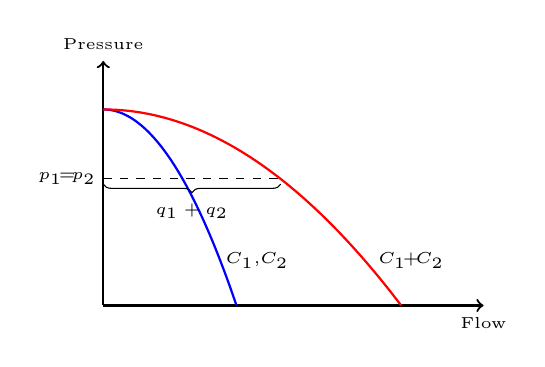
\begin{tikzpicture}[scale=1.15,transform shape]

      \draw[->][thick] (0,0) -- (4.2,0) node[below] {\tiny Flow};
 \draw[->][thick] (0,0) -- (0,2.7) node[above] {\tiny Pressure};
      \draw[scale=0.5,domain=0:2.94,smooth,variable=\x,blue,thick] plot ({\x},{4.33-0.5*\x*\x});
      \draw[scale=0.5,domain=0:6.58,smooth,variable=\x,red,thick] plot ({\x},{4.33-0.1*\x*\x});
    
    
    
\draw [dashed](0,1.4) -- (1.96,1.4);
\node at (-0.4,1.4) {\tiny $p_1$\!=\!$p_2$};
\node at (1.7,0.5) {\tiny $C_1$,$C_2$};
\node at (3.4,0.5) {\tiny $C_1$\!+\!$C_2$};


\draw [decorate,decoration={brace,amplitude=3pt,mirror,raise=2pt},yshift=0pt]
(0,1.4) -- (1.96,1.4) node [black,below,midway,xshift=0.0cm,yshift=-0.15cm] {\tiny $q_1+q_2$};
\end{tikzpicture} 
\caption{Two pumps connected in parallel with the same performance curves.}
\label{fig:parallelpumpcurve}
\end{figure}

\vspace{-3mm}

Additionally, a system configuration with parallel pumps provides flexibility by permitting the switching of parallel pumps on or off in order to adjust to varying demands in the network. 

\subsection{Valves}
\label{valves}

Along with pumps, valves can be also seen as actuators. Unlike pumps, valves are passive actuators in the sense that they do not consume energy. In principle, there exist many types of different valves. They can be categorized as non-return valves, control valves, shut-off valves and the combination of the two former one. Non-return valves allow flow only in one direction, while control valves can either adjust the flow or the pressure on the two endpoints. The former category is typically called a Flow Control Valve(FCV), while the latter is called a Pressure Reducer Valve or Pressure Regulating Valve(PRV). Shut-off valves are important components of the network since they can change the structure of the system, when for instance the network is under maintenance or the flow is being redirected. By closing a valve in the system, certain parts of the network can be isolated.

\section{Description summary}
\label{distribution_system_solutions}

As it has been explained in \secref{pipe_networks}, WSSs can have different structure, complexity, they can operate according to different rules and can consist of different hydraulic components. The main structural and operational differences between drinking water networks are typically due to the differences in the landscape and due to the different types of end-user water consumptions. The main purpose of such systems, however, is usually the same; to maintain the water at positive pressure in order to ensure that water reaches all parts of the network, that a sufficient flow is available and to ensure that untreated water cannot enter the network. 

In Denmark, the water is typically pressurised by pumps that pump water into WTs, constructed at the highest local point in the network, if possible. In such systems, in order to find an efficient and safe operation, unique solutions are required. Therefore, the following discussion focuses on the introduction of the Randers WSS, in order to get an overview of the operation and to explain the structural and physical properties of the network which are later used for modelling purposes. 

\newpage

\section{The Randers water supply network}
\label{the_randers_water_supply_network}

The Randers drinking WSS is managed by Verdo A/S, which is the main supplier of drinking water and heating to the city of Randers. Verdo supplies water to approximately 46.000 customers in the municipality \cite{verdo}. The WSS is a complex, mixed loop and tree configuration with many different distribution areas. The coverage of the distribution areas is shown in \figref{fig:level_zones}.

%illustration of distribution regions in Randers
\begin{figure}[H]
\centering
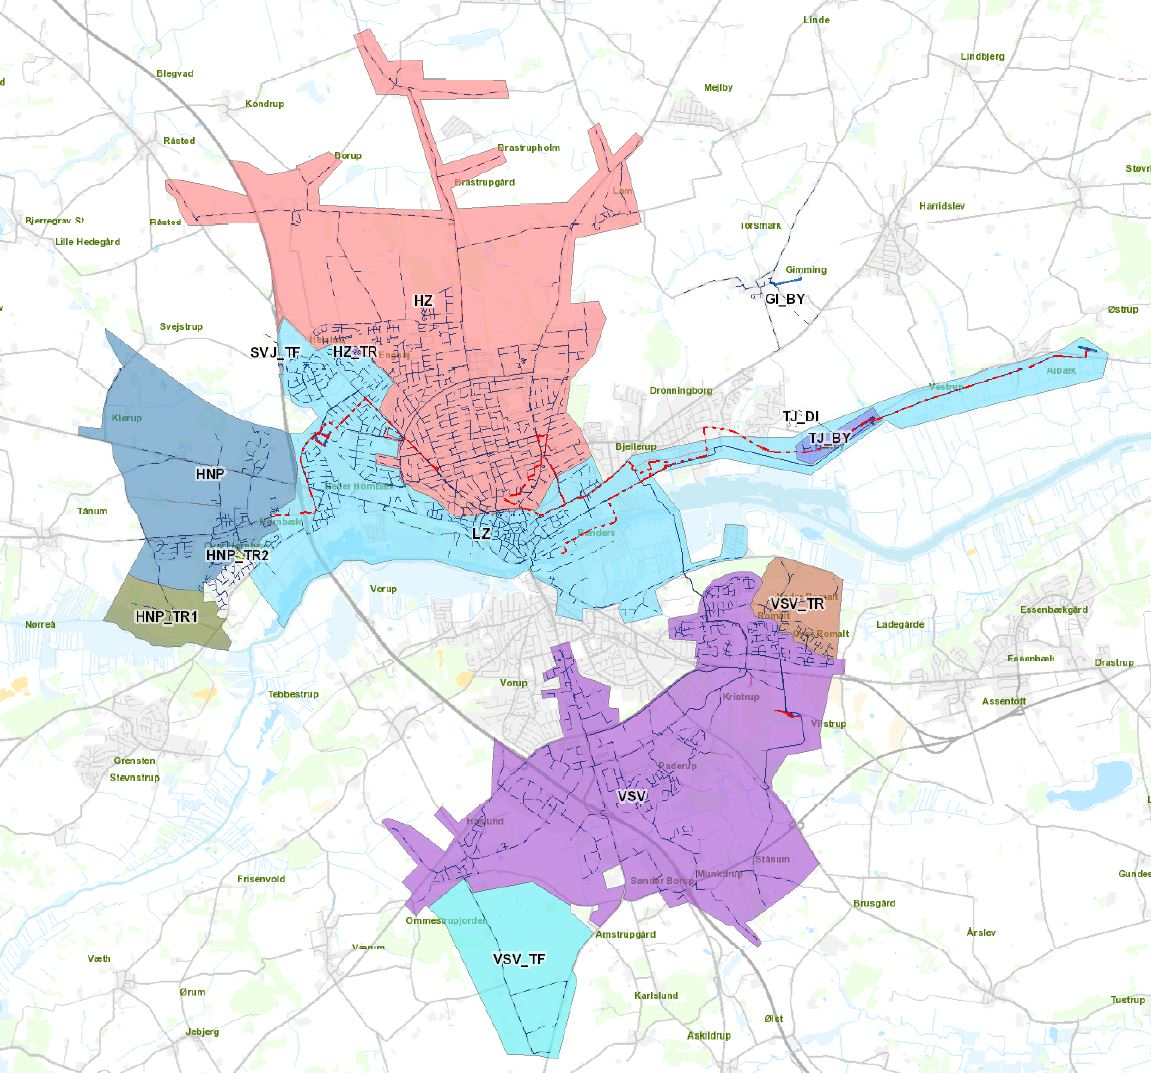
\includegraphics[width=0.9\textwidth]{report/pictures/level_zones}
\caption{Distribution zones in the Randers WSS \cite{verdo}.}
\label{fig:level_zones}
\end{figure}

\vspace{-3mm}

Although the network consists of many different distribution zones, the distribution in the city can be split into four main areas regarding the different geographical properties of the landscape. Randers can be split into two regions, Randers North and Randers South. This is due to the fact that Randers fjord divides the city into a northern and a southern half \cite{verdo}. Furthermore, it is important to note that the distribution coverage illustrated in \figref{fig:level_zones}, describes the network in its form from the year 2013. Since 2013, additional pipelines and smaller distribution areas have been added to the network, meaning that Verdo's supply network has grown during the past few years. Although the structure has slightly changed, the main water works and pumping stations are still the same, therefore the characteristics and operation of the network has not changed significantly. Consequently, the structure of the network is considered to be sufficiently updated for modelling and control purposes. 

The distribution network which is located in the southern part of the city is called Vilstrup. This zone has its own waterwork and pumping station which makes it possible to supply the whole Randers South by itself. The distribution area on the southern part to Randers fjord consists of this zone, with one water work and with the corresponding pumping station. Vilstrup is shown in \figref{fig:vilstrup_region}.

\begin{figure}[H]
\centering
\begin{subfigure}{.49\textwidth}
\centering
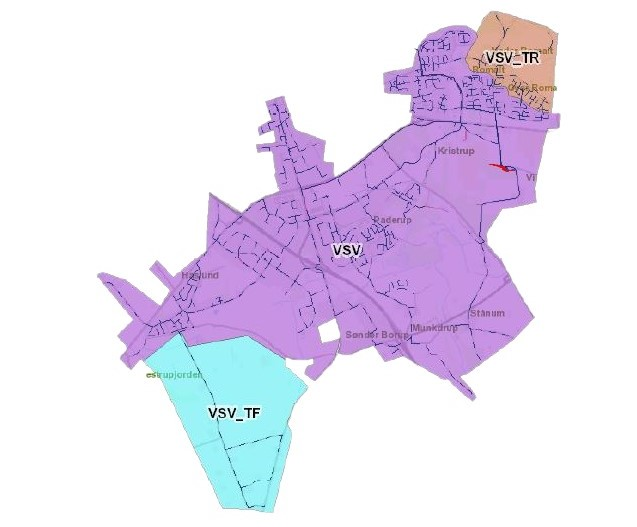
\includegraphics[width=0.5\textwidth]{report/pictures/Vilstrup_region}
  \caption{Vilstrup.}
  \label{fig:vilstrup_region}
\end{subfigure}
\begin{subfigure}{.49\textwidth}
\centering
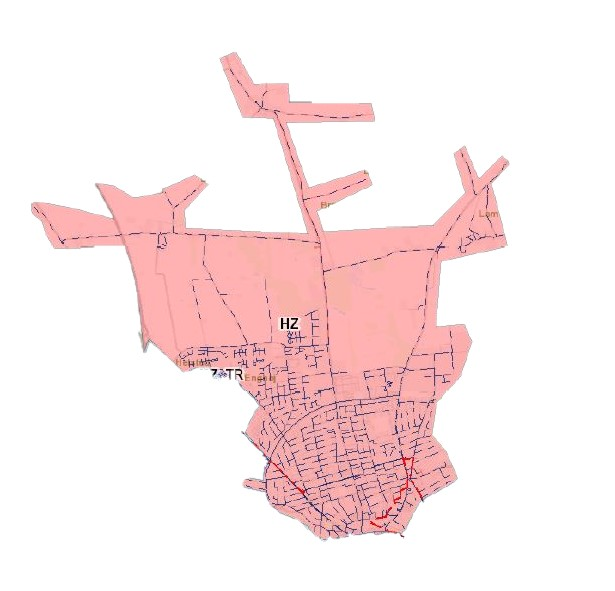
\includegraphics[width=0.5\textwidth]{report/pictures/Highzone_region}
  \caption{High Zone.}
  \label{fig:highzone_region}
\end{subfigure}
\caption{Geographical illustration of Vilstrup and High Zone distribution areas in Randers.}
\label{fig:vsv_hz_pic}
\end{figure}

\vspace{-3mm}

% %Vilstrup region
% \begin{figure}[H]
% \centering
% 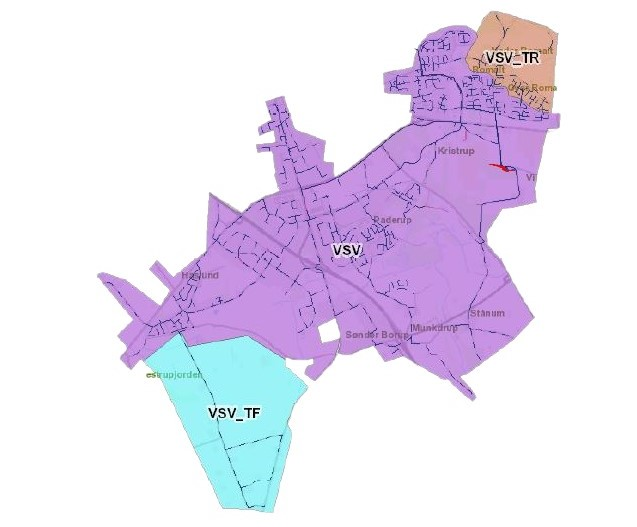
\includegraphics[width=0.35\textwidth]{report/pictures/Vilstrup_region}
% \caption{Vilstrup zone in Randers.}
% \label{fig:vilstrup_region}
% \end{figure}

The connection between Vilstrup and Randers North is through an emergency line, which is  used in emergency cases when the waterwork and pumping station in Vilstrup malfunctions or if there is a contamination in the WTs in Randers South. In these cases waterworks from the northern parts can provide water. An emergency case is for instance when the drilled water in the water works becomes contaminated due to the intensive farming activity in this area. It is important to note that the emergency line is closed in most of the time by a valve, however this valve opens every night for approximately one hour to let the stored water out from this pipeline. It is necessary to let fresh water through every day, since otherwise there is a risk that water quality falls below the accepted level. Besides the emergency cases, the  water distribution in Vilstrup does not rely on the waterworks and pumping stations in Randers North.  

Randers North consists of three different areas, each having their own particular geographical properties. The water distribution in these regions are strongly related to each other, meaning that the pump schedules rely on the water levels in the WTs and on the end-user consumption in the different regions. 

The area shown in \figref{fig:highzone_region} above is called the High Zone(HZ) due to the high elevation level of the region. This part of the city lies approximately 55 meters above sea level, which means that high pumping effort is required to deliver the pressurised water here. Furthermore, this area has mainly a grid structure with several loops, which is due to the fact that the city center lies on this part of the city.  

The area underneath the HZ is called the Low Zone(LZ). This area in Randers lies approximately on sea level. Therefore, the HZ and LZ have a significant elevation difference which requires special pumping solutions in this area. In order to get a visual overview of the geographical properties of the HZ and LZ, elevation profiles are shown between these two areas in \appref{elevation_profile_of_randers}, in \figref{fig:elev_profile} and \figref{fig:elev_profile1}. The LZ area is illustrated in \figref{fig:lowzone_region}.

\begin{figure}[H]
\centering
\begin{subfigure}{.49\textwidth}
\centering
\hspace{3mm}
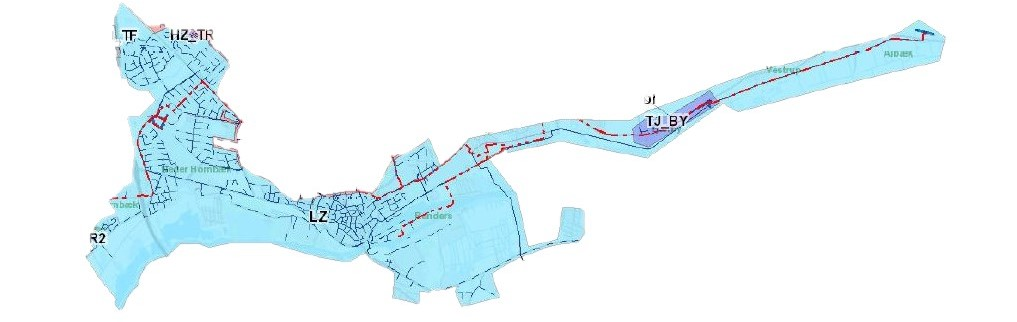
\includegraphics[width=1.1\textwidth]{report/pictures/Lowzone_region}
\vspace{2mm}
  \caption{Low Zone.}
  \label{fig:lowzone_region}
\end{subfigure}
\begin{subfigure}{.49\textwidth}
\centering
\hspace{3mm}
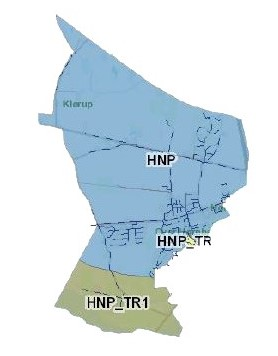
\includegraphics[width=0.35\textwidth]{report/pictures/Hornbaek_region}
  \caption{Hornbæk.}
  \label{fig:hornbaek_region}
\end{subfigure}
\caption{Geographical illustration of Low Zone and Hornbæk distribution areas in Randers.}
\label{fig:lz_hbp_pic}
\end{figure}
\vspace{-3mm}

The fourth main area in the Randers WSS is an area, which according to its elevation, neither belongs to the HZ, nor to the LZ. This area is called Hornbæk and shown in \figref{fig:hornbaek_region}. The elevation in this area is around 30 meters above sea level and lies in the western part of the city. This zone is connected to the rest of the distribution network through a transmission line and the structure is mainly a tree configuration. 

\subsection{Waterworks and pumping stations}
\label{waterworks_and_pumping_stations}

Verdo provides drinking water by pumping water from groundwater bases and treating the water in four different water works. Due to the high quality of ground water, this water treatment is only an aeration process in all areas, except the Vilstrup zone. In Vilstrup, as mentioned above, farming activity is high, therefore the water gets contaminated very often. 

The WSS in Randers has four waterworks and four pumping stations, located in different locations points in the city. In order to draw a better picture and to introduce the corresponding pumping stations and water works in a simple way, they are listed and labelled according to their names and their geographical locations and properties are described. The water works and pumping stations are listed in \tabref{waterworks_tab} and \tabref{pumpingstations_tab}, respectively.

\begin{table}[!htp]
\begin{subtable}{.52\linewidth}
\begin{center}
    \begin{tabular}{| l | l | l |}
    \hline
    BKV & Bunkedal Water work   \\ \hline
    ØSV & Østrup Skov Water work  \\ \hline
    VSV & Vilstrup Water work  \\ \hline
    OMV & Oust Mølle Water work   \\
    \hline
    \end{tabular}
\end{center}
\vspace{-3mm}
\caption{Waterworks.}
\label{waterworks_tab}
\end{subtable}
\begin{subtable}{.4\linewidth}
\begin{center}
    \begin{tabular}{| l | l | l |}
    \hline
    HBP & Hobrovej Pumping Station   \\ \hline
    HSP & Hadsundvej Pumping Station  \\ \hline
    TBP & Toldbodgade Pumping Station  \\ \hline
    HNP & Hornbæk Pumping Station   \\
    \hline
    \end{tabular}
    \end{center}
\vspace{-3mm}
\caption{Pumping stations.}
\label{pumpingstations_tab}
\end{subtable}
\end{table}
\vspace{-3mm}

In order to show the geographical location of the waterworks and pumping stations, an illustration of the network is shown, where each pumping station and waterwork are labelled with the abbreviation of their names. It is also necessary to illustrate, which station belongs which supply zones. The illustration is shown in \figref{fig:pumping_stations_and_waterworks}.

\vspace{-5mm}

  %Pumping stations and waterworks in Randers
\begin{figure}[H]
\centering
%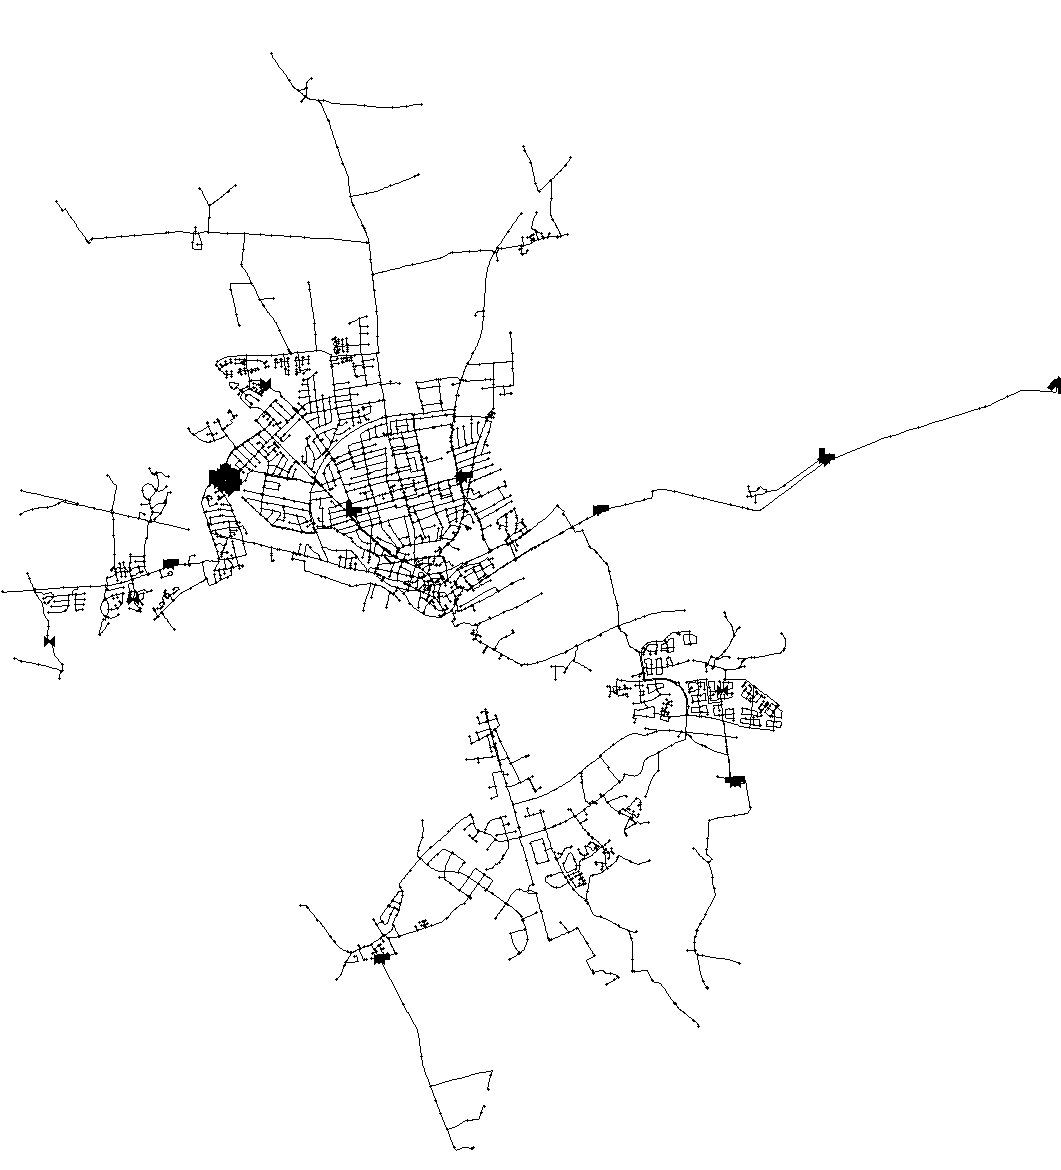
\includegraphics[width=1\textwidth]{report/pictures/verdo_pic}
 \begin{tikzpicture}[scale=0.65,transform shape]
     \node at (0,0) {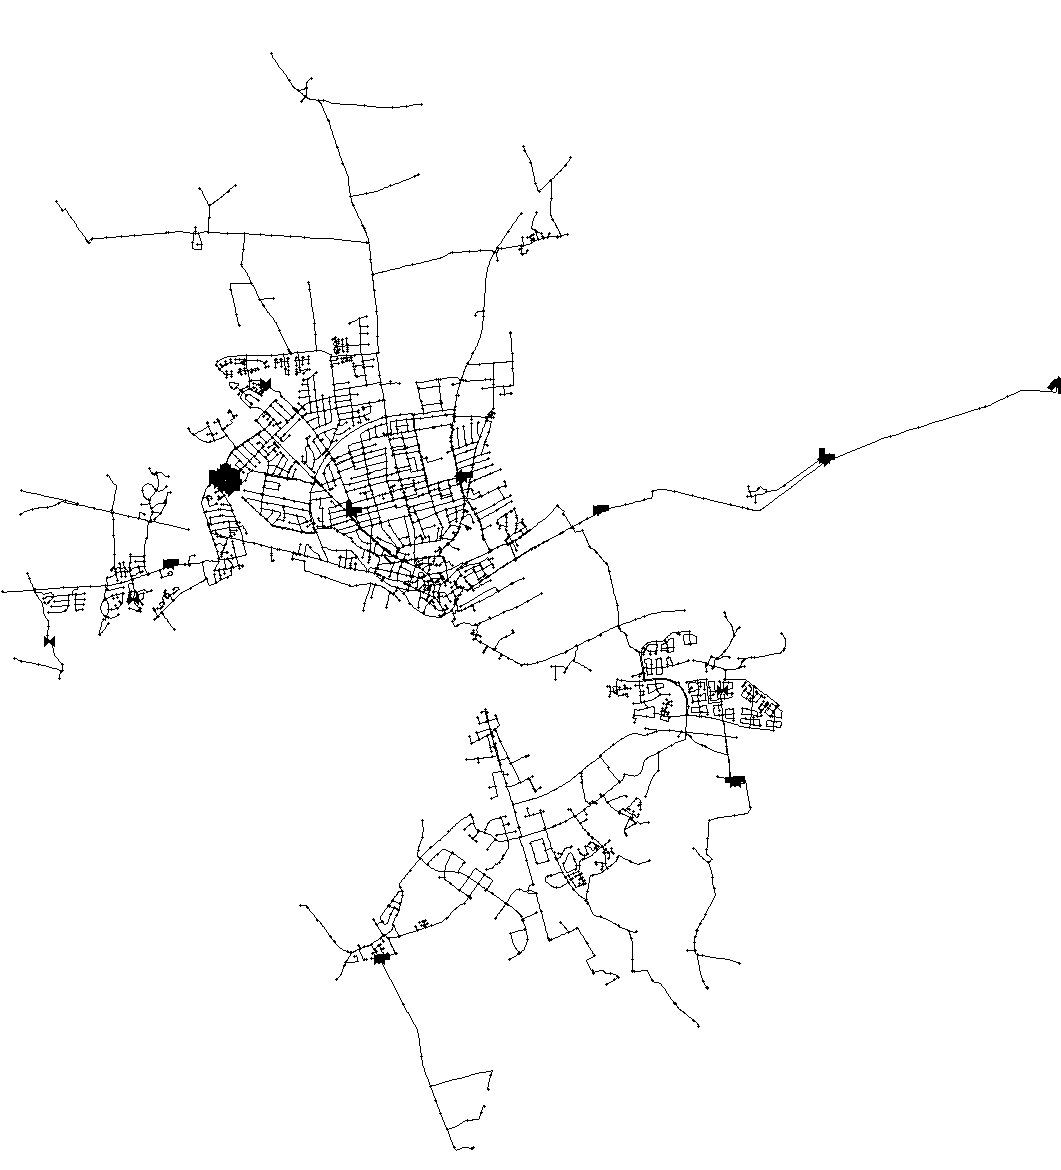
\includegraphics[width=1.5\textwidth]{report/pictures/verdo_pic}};

%     \node[anchor=south west,inner sep=0] at (0,0) {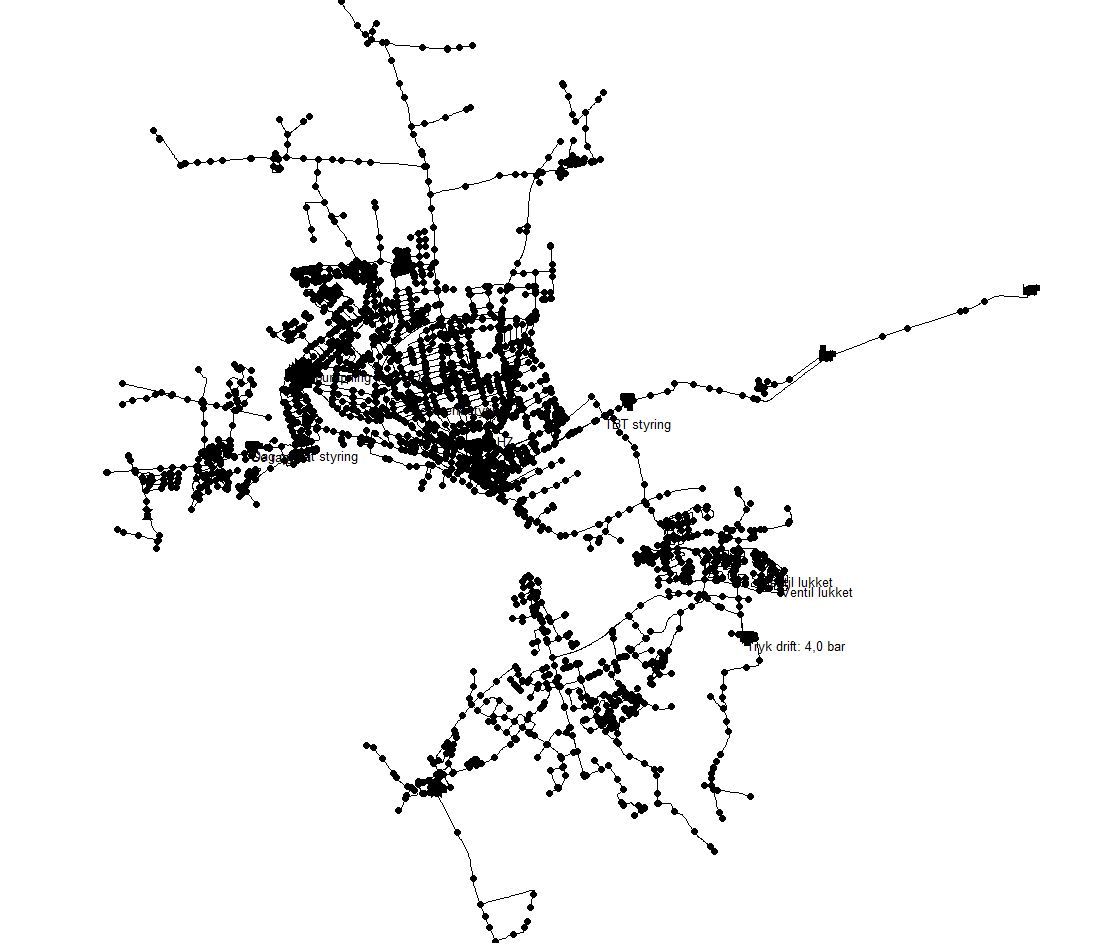
\includegraphics[width=\textwidth]{report/pictures/verdo_pic1}};
            \draw[blue,ultra thick,rounded corners] (3.55,-4.55) rectangle (4.75,-3.7);
             \draw[blue,ultra thick,rounded corners] (5.55,2.15) rectangle (6.8,3);
                      \draw[blue,ultra thick,rounded corners] (-7,2.65) rectangle (-5.75,1.8);
              \draw[blue,line width=0.65mm,rounded corners] (10.05,4.35) rectangle (11.25,3.55);
 \node[black] at (6.05,3.5) {\Large Bunkedal};
   \node[black] at (10.55,4.8) {\Large Østrup Skov};
      \node[black] at (5.6,-4.85) {\Large Vilstrup};
     \node[black] at (-8.55,3) {\Large Oust Mølle};
     
     \draw[red,ultra thick,rounded corners] (-2.1,1.85) rectangle (-0.9,2.7);
      \draw[red,ultra thick,rounded corners] (-8,-0.15) rectangle (-6.8,0.7);
           \draw[red,ultra thick,rounded corners] (1.05,1.15) rectangle (2.25,2);
                \draw[red,ultra thick,rounded corners] (-4.35,1.2) rectangle (-3.15,2.05);
                
                 \node[black] at (2.6,0.65) {\Large Toldbodgade};
                 \node[black] at (0.45,2.85) {\Large Hadsundvej};
                 \node[black] at (-6.45,-0.5) {\Large Hornbæk};
                    \node[black] at (1,5) {\Large Hobrovej};
     
 \draw [-latex](0.1,4.7) -- (-3.25,2.35);
\end{tikzpicture}
 
\caption{Water works(encircled in blue) and Pumping stations(encircled in red).}
\vspace{-3mm}
\label{fig:pumping_stations_and_waterworks}
\end{figure}

The main water works in Randers North are Oust Mølle, Bunkedal and Østrup Skov. In the two latter ones, the quality of water is very good. This is due to the fact that the groundwater lies under the ground such that it is protected by certain ground layers. These layers make it possible to distribute the water without any kind of cleaning process, except aeration. These protection layers have been created by Randers fjord due to glacial erosion over the past few centuries \cite{geological1909water}. In this case, contamination by farming is not an option since these drilling stations are located very close to the fjord and therefore considered as reliable groundwater sources. 

One of the drawbacks, however, is that the fresh water sources are located in the LZ. Therefore, the water has to be pumped from BKV, ØSV and OMV to locations with higher elevation. Since BKV, ØSV and OMV are the main sources to the HZ and LZ areas, in some cases water has to be pumped to approximately 50 meters above sea level. For this reason, Toldbodgade(TBP) pumping station and the puming station in OMV provide the pressurized water to other pumping stations and to the corresponding WTs in the HZ area. In the HZ, at the border of the LZ and HZ, two pumping stations are located. These pumping stations, Hadsundvej(HSP) and Hobrovej(HPB), pump the water towards the grid in the HZ areas. The water is delivered with the help of transmission lines from the three main water works in the LZ to HSP and HBP. 

As can be seen in \figref{fig:pumping_stations_and_waterworks}, and as mentioned previously, the structure of the network in the HZ is a grid. The two main pump stations, HSP and HBP provide the pressure and flow to this grid, such that they keep a balance in pressure and flow. Furthermore, there are WTs placed both at HSP and HBP. The main supply stations, OMV and TBP in the LZ operate such that the pumps are controlled according to the water level in the WTs in HBP and HSP, respectively. Since the HZ has an elevation of approximately 50 meters, the static pressure in each WT at the two pumping stations is sufficient to provide pressure in the LZ areas, without any pumping effort when the main supply pumps HBP and TBP are turned off. Therefore, the WTs provide pressure to the LZ areas such that the geodesic properties are exploited. An illustration of the two pumping stations and the HZ grid is shown in \figref{fig:HBP_HSP_grid}. 

 %HZ grid
\begin{figure}[H]
\centering
%
\includegraphics[width=0.4\textwidth]{report/pictures/missingfigure}
 \usetikzlibrary{arrows}
\begin{tikzpicture}[scale=1.1,transform shape]



\draw [thick](-3.7,1.4) -- (0.1,1.4);
\draw [thick](-3.7,1) -- (0.1,1);
\draw [thick](-3.7,0.6) -- (0.1,0.6);
\draw [thick](-3.7,0.2) -- (0.1,0.2);
\draw [thick](-3.3,1.8) -- (-3.3,0.2);
\draw [thick](-2.8,1.8) -- (-2.8,0.2);
\draw [thick](-2.3,1.8) -- (-2.3,0.2);
\draw [thick](-1.8,1.8) -- (-1.8,0.2);
\draw [thick](-1.3,1.8) -- (-1.3,0.2);
\draw [thick](-0.8,1.8) -- (-0.8,0.2);
\draw [thick](-0.3,1.8) -- (-0.3,0.2);

%pump
\node[thick][draw,circle,minimum size=0.4cm] (p0) at (-3,-0.5) {};
\node(p1) at ($(p0)+(-0.2,0)$) {};
\node(p2) at ($(p1)+(0.2,0.2)$) {};
\node(p3) at ($(p1)+(0.4,0)$) {};
\draw [thick](p1.center) -- (p2.center) -- (p3.center);

%pump
\node[thick][draw,circle,minimum size=0.4cm] (p0) at (-0.6,-0.5) {};
\node(p1) at ($(p0)+(-0.2,0)$) {};
\node(p2) at ($(p1)+(0.2,0.2)$) {};
\node(p3) at ($(p1)+(0.4,0)$) {};
\draw [thick](p1.center) -- (p2.center) -- (p3.center);


\draw [thick](-0.6,-0.3) -- (-0.6,0.2) -- (-3,0.2) -- (-3,-0.3);
\draw [thick] (-3.3,-1.1) rectangle (-2.7,-1.5);
\node at (-3,-1.3) {\tiny HBP};
\draw [thick] (-0.9,-1.1) rectangle (-0.3,-1.5);
\node at (-0.6,-1.3) {\tiny HSP};
\node at (-1.1,-2.6) {\tiny LZ};
\node at (0.5,0.9) {\tiny HZ};
\draw [thick](-3,-0.7) -- (-3,-1.1);
\draw [thick](-0.6,-0.7) -- (-0.6,-1.1);
\draw [thick](-3,-1.5) -- (-3,-1.7) -- (-0.6,-1.7) -- (-0.6,-1.5);
\draw [thick](-1.8,-1.7) -- (-1.8,-3.1);
\draw [thick](-2.1,-2.5) -- (-1.5,-2.2);
\draw [thick](-2.1,-2.8) -- (-1.5,-2.5);
\draw [thick](-2.1,-3.1) -- (-1.5,-2.8);
\draw [thick](-0.3,-1.3) -- (0.2,-1.3) -- (0.2,-1.2);
\draw [thick] (0,-0.7) rectangle (0.4,-1.2);
\draw [fill=cyan] (0,-0.9) rectangle (0.4,-1.2);

\draw [thick](-3.3,-1.3) -- (-3.8,-1.3) -- (-3.8,-1.2);
\draw [thick] (-4,-0.7) rectangle (-3.6,-1.2);
\draw [fill=cyan] (-4,-0.9) rectangle (-3.6,-1.2);
\end{tikzpicture}
\caption{Hadsundvej and Hobrovej pumping stations with the HZ grid and LZ.}
\label{fig:HBP_HSP_grid}
\end{figure}

\vspace{-3mm}

As can be seen in \figref{fig:HBP_HSP_grid}, the pumping stations with the WTs are connected through the grid, furthermore the WTs are connected in the LZ area.

In order to avoid too high or too low pressure in the system, the pressure needs to be controlled in one pumping station and the flow in the other one. HBP is responsible for flow control, while HSP is responsible for the pressure control. Thereby it is avoided to provide too high flow or too low or high pressure to the end-users. 

One special case of the operation which explains well the behaviour of the tanks located in the HZ, is when the supply pump stations, TBP and OMV are both turned off. In this case, the tanks are being emptied and all the static pressure stored in the tanks is being used to supply the LZ. \figref{fig:pressure_balance_Randers} shows an illustration for the pressure balance in the tanks.

 %tank emptying
\begin{figure}[H]
\centering
%
\includegraphics[width=0.4\textwidth]{report/pictures/missingfigure}
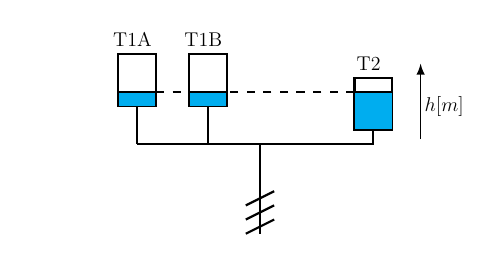
\begin{tikzpicture}[scale=0.6,transform shape]

\draw [thick](-2.5,-1.95) -- (-2.5,-3.4);
\draw [thick](-2.8,-2.8) -- (-2.2,-2.5);
\draw [thick](-2.8,-3.1) -- (-2.2,-2.8);
\draw [thick](-2.8,-3.4) -- (-2.2,-3.1);
\draw [thick] (-0.5,-0.1) rectangle (0.3,-1.2);
\draw [fill=cyan] (-0.5,-0.4) rectangle (0.3,-1.2);
\draw [thick] (-4,0.4) rectangle (-3.2,-0.7);
\draw [fill=cyan] (-4,-0.4) rectangle (-3.2,-0.7);
\node at (-5.2,0.7) {\large T1A};
\node at (-3.7,0.7) {\large T1B};
\node at (-0.2,0.2) {\large T2};
\node at (1.4,-0.7) {\large $h [m]$};
\draw [dashed](-0.5,-0.4) -- (-3.2,-0.4);
\draw [dashed](-4.7,-0.4) -- (-4,-0.4);
\draw [thick] (-5.5,0.4) rectangle (-4.7,-0.7);
\draw [fill=cyan] (-5.5,-0.4) rectangle (-4.7,-0.7);
\node at (-7.3,-1.5) {};
\draw [thick] (-0.1,-1.2) -- (-0.1,-1.5) -- (-3.6,-1.5)  -- (-3.6,-0.7) --(-3.6,-1.5) node (v2) {} (-5.1,-1.5) node (v1) {} -- (-5.1,-0.7);
\draw  [thick] (v1);
\draw  [thick](-5.1,-1.5)--(-3.6,-1.5);
\draw  [thick](-2.5,-1.5) -- (-2.5,-2.2);
\draw [-latex](0.9,-1.4) -- (0.9,0.2);
\end{tikzpicture}
\caption{Pressure balance in the elevated reservoirs in the HZ. }
\label{fig:pressure_balance_Randers}
\end{figure}

\vspace{-3mm}
It is important to note, however, that it requires a long time for balancing out the levels in the WTs. In some cases the goal is to empty the tanks in the HZ due to maintenance. In this case, it can take up to 12 hours for the WTs to be empty.  

Furthermore, in Hornbæk, the elevation is above sea level, therefore the static pressure from the two main pumping stations are not sufficient to supply the area. Due to this, boosting is needed. The HNP pumping station in Hornbæk boosts the pressure of the water, coming from OMV. 

\subsection{Control perspectives}
\label{Randers_wss_summary}

As it has been described in \secref{the_randers_water_supply_network}, Vilstrup is an individual distribution area if normal operation is assumed. Therefore, VSV is able to provide the total consumption demand in Randers South, without the help of the other waterworks in Randers North. Consequently, the WSS in Randers South can be separated when the water management in Randers North is being analysed. The network in Randers North, with the corresponding water works, WTs and pumping stations is shown in \figref{fig:simplified_network}. 

%Simplified network map
\begin{figure}[H]
\centering
\usetikzlibrary{arrows}
\begin{tikzpicture}[scale=0.8,transform shape]

 \node[anchor=south west,inner sep=0] at (0,0) {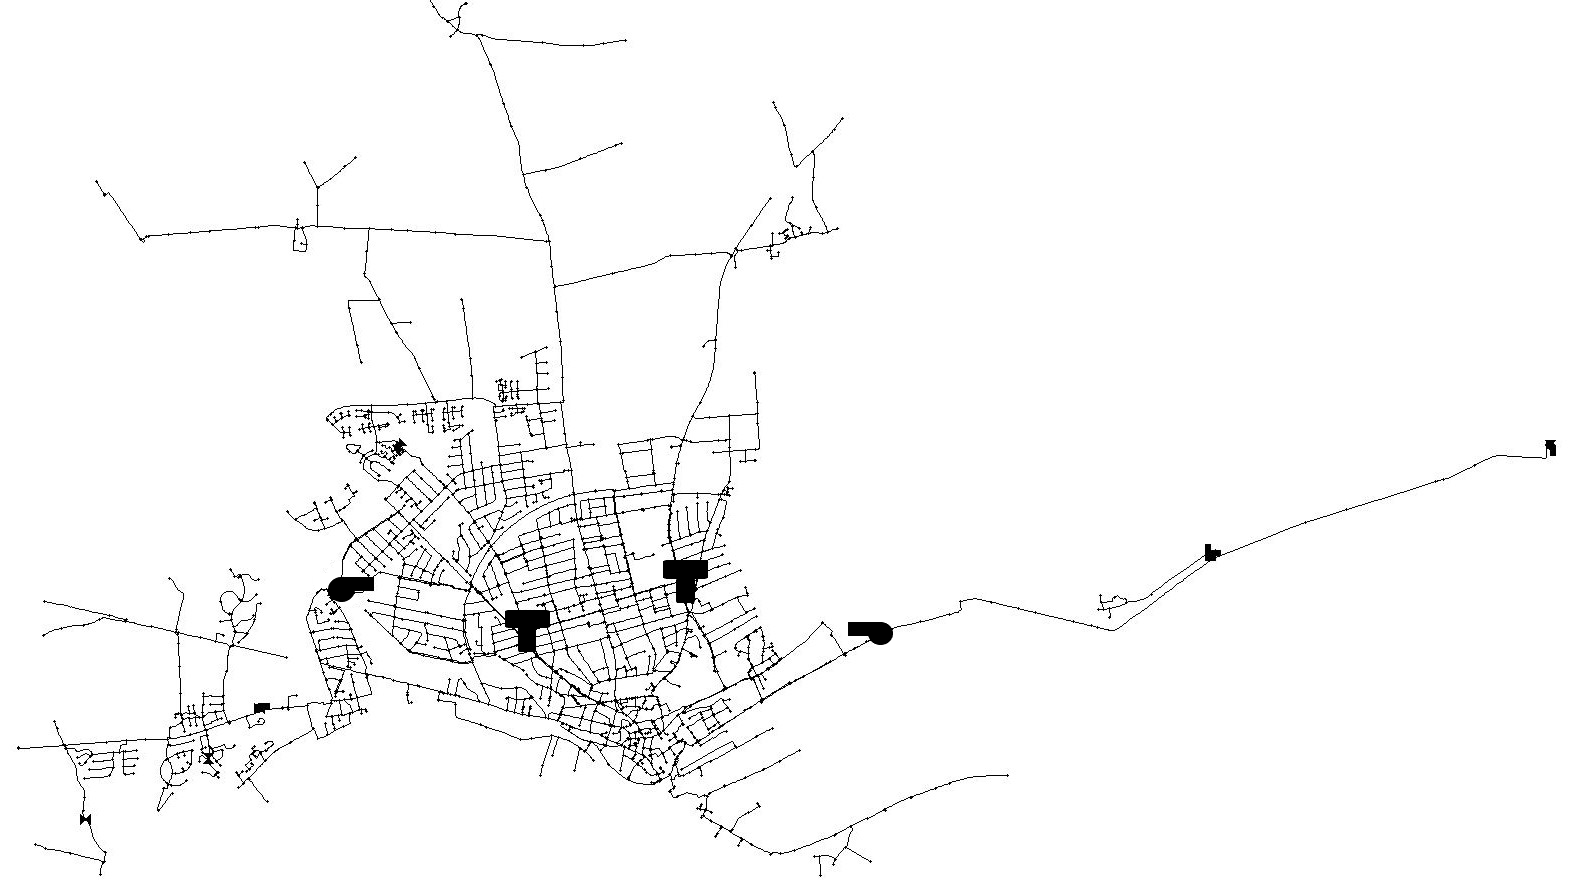
\includegraphics[width=\textwidth]{report/pictures/verdo_pic3}};
\node[black] at (7.2,3.1) {\footnotesize HSP};
\node[black] at (8.9,2.1) {\footnotesize TBP};
\node[black] at (2.8,3.2) {\footnotesize OMV};
\node[black] at (4.6,1) {\footnotesize HBP};
\draw [-latex][thick](4.9,2.2) -- (4.6,1.3);
\end{tikzpicture}


%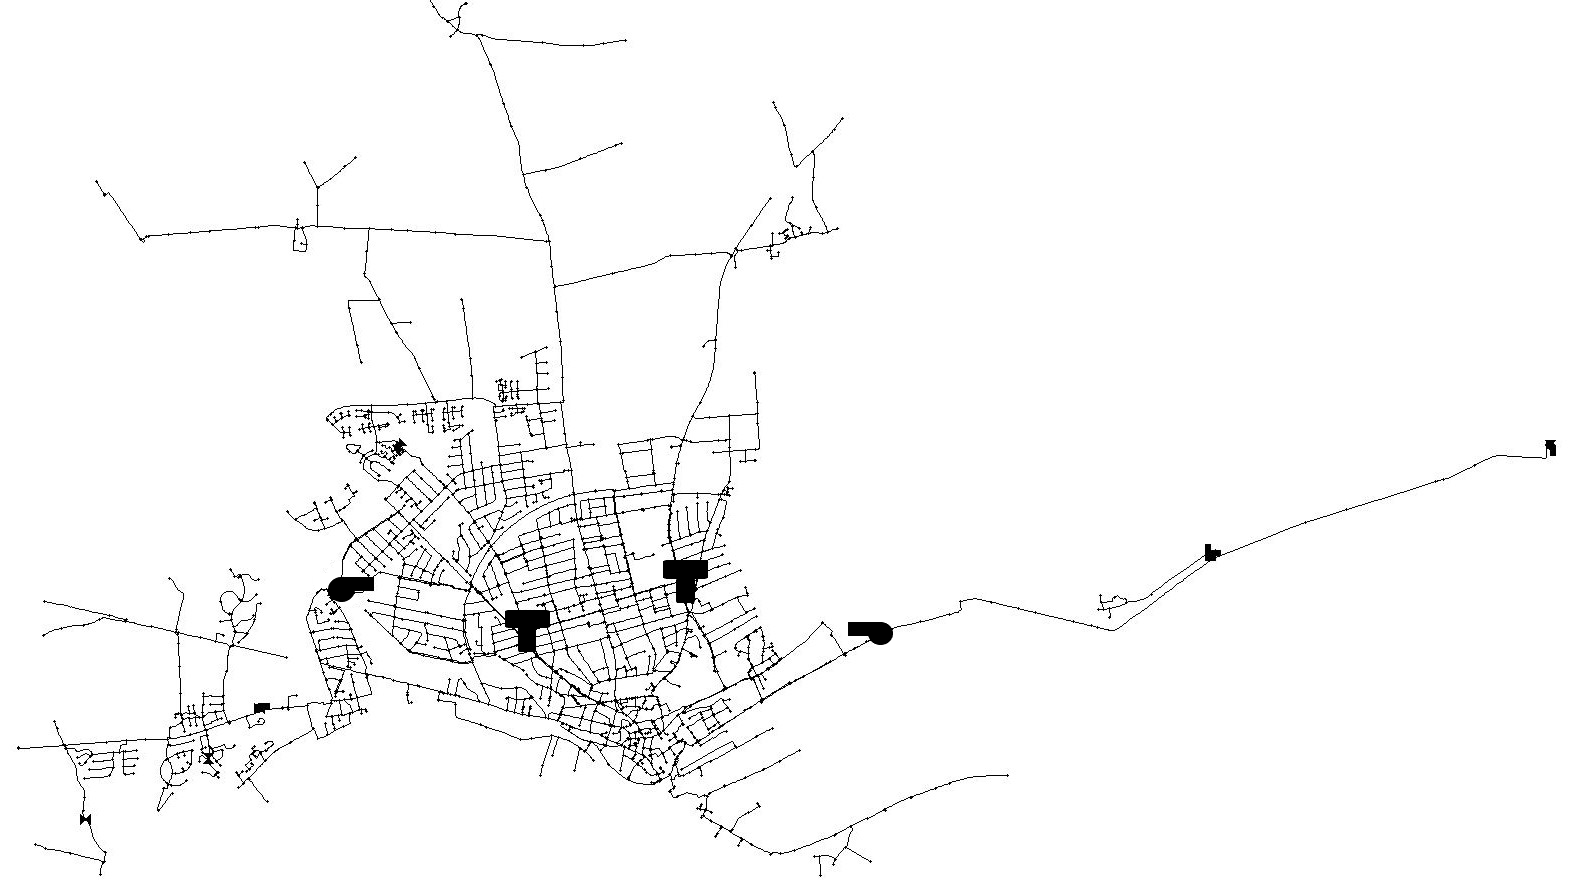
\includegraphics[width=0.95\textwidth]{report/pictures/verdo_pic3}
\caption{The network map of Randers North.}
\label{fig:simplified_network}
\end{figure}
\vspace{-3mm}

In Randers North the control is focused on the two main pumping stations, TBP and OMV. Both pumping stations are operated by controlling the flow according to the water level in the corresponding WTs in HBP and HSP. TBP pumping station delivers the water coming from the two waterworks BKV and ØSV. In HBP and HSP, pressure and flow controlled pumps keep the pressure-flow balance in the grid. Furthermore, the distribution zone called HNP is seen as a region, where the booster pumps deliver the water mainly from OMV. 

The available model of the system is going to be used for control purposes, which means that the model for control needs to be simple, however needs to have the same characteristics as of the original network. In the Randers WSS, the purpose of control is to find an optimal control scheme which is able to actuate the pumps at the two main pumping stations HSP and HBP, such that the dynamic effect of the WTs at each station are utilized. Challenges of control come up due to the multiple WTs in the system, actuated by multiple pumping stations. In order to create a framework which is commissionable for optimal control, first the mathematical description of the model is required. 

\section{Simulation framework in EPANET}
\label{simulation_framework_in_EPANET}

The main properties of the Randers WSS has been discussed in \secref{the_randers_water_supply_network}. In order to draw a better picture of the simulation framework in EPANET, the structure of the model, the data and certain abstractions made throughout the simulation is going to be discussed. 

\subsection{Model and data structure}
\label{model_data_and_structure}

As it has been explained in \chapref{description_of_water_supply_systems}, the typical components of WSSs are: reservoirs, pipes, pumps and valves. For simulation purposes, it is necessary that the model of the real-world network consists of thousands of elements in order to accurately mimic hydraulic behaviour and to replicate the topographical layout of the system. Such models are appropriate for simulation purposes, however, they are too complex for demanding online optimisation tasks. However, the available data and information in EPANET can be used to create a reduced order model for control purposes. 

The use of Geographic Information Systems(GIS) and Supervisory Control and Data Acquisition(SCADA) systems in the water industry resulted in an increasing amount of information about actual network topology and service that can be utilized in a hydraulic network model \cite{johnson2016geographic}. Consequently, the simulation model of WSSs include almost exactly the same amount of components as in real-life. The following data and model description strongly relies on the documentation of the Randers WSS EPANET model \cite{verdo_doc}, provided by Verdo A/S, where the main modelling steps are explained. The model is mainly based on the data stored in GIS and the SCADA system, however different case studies and experience have also been incorporated into the model. It is important to note that the following results and properties of the EPANET model serve as a basis for understanding the data processing and therefore the discussion is important in the thesis.  

Initially, during the modelling, nodes have been made between each different pipe elements. However with large number of elements, calculation time has been increasingly high. Therefore, the number of nodes in the network have been reduced based on the fact that pipe sections with the same material and dimensions can be treated as one pipeline. In order to illustrate the complexity of the network, the number of elements in the simulation model, including the VSV region, is shown in \tabref{numberofelements_table}.

\begin{center}
\label{numberofelements_table}
    \begin{tabular}{ | p{3cm} | p{3cm} |}
    \hline
    \textbf{Element type} & \textbf{Number}  \\ 
    \hline
    Links & 4144  \\ 
    \hline
    Nodes & 4180  \\ 
    \hline
    Tanks & 6  \\ 
    \hline
    \end{tabular}
    \captionof{table}{Number of WSS elements.}
\end{center}

\vspace{-3mm}

When the EPANET simulation network is considered, it is important to state that certain parts do not reflect the structure of the real-world network. Due to these abstractions the exact structure and operation does not necessarily reflect the real-world configuration. However, both the simulation and measurement data on which the model relies provide similar results. Therefore, for instance, the number of WTs in the model does not necessarily match the number of WTs in the real system. Water works usually have large WTs, where the aeration process and filtering is being done, however in certain parts of the model, water works do not use these WTs. Furthermore, the number of pumps at certain pumping stations is not the same as in real world, since the model has been done such that the overall pumping effort is considered.  

\subsection{Water consumption data}
\label{water_consumption_data}

In the EPANET model, the consumption is divided into two groups: non-industrial and industrial water consumption. It has been chosen to keep the number of demand categories low, as it turned out that the quality of the data from GIS is not representative. Among many reasons, this is due to the fact that, for instance, one-storey buildings and two-or more-storey buildings have very similar consumption rates. The consumption curves have been defined such that they match the pumped water volumes from waterworks and pumping stations in each individual zone. Therefore, a calculation has been made which shows the deviation of the consumption over the day. Thereby, it has been possible to see the uniformity of the consumption types in each zone \cite{verdo_doc}. With around three percent uncertainty, the consumption patterns turned out to be representative in the model. The demand patterns over a 24 hours long period are periodic. The pattern of the water consumption deviation is shown in \figref{fig:demandpatterns_EPANET} .

\begin{figure}[H]
\centering
%
\includegraphics[width=0.4\textwidth]{report/pictures/missingfigure}
% This file was created by matlab2tikz.
%
%The latest updates can be retrieved from
%  http://www.mathworks.com/matlabcentral/fileexchange/22022-matlab2tikz-matlab2tikz
%where you can also make suggestions and rate matlab2tikz.
%
\definecolor{mycolor1}{rgb}{0.00000,0.44700,0.74100}%
\definecolor{mycolor2}{rgb}{0.85000,0.32500,0.09800}%
%
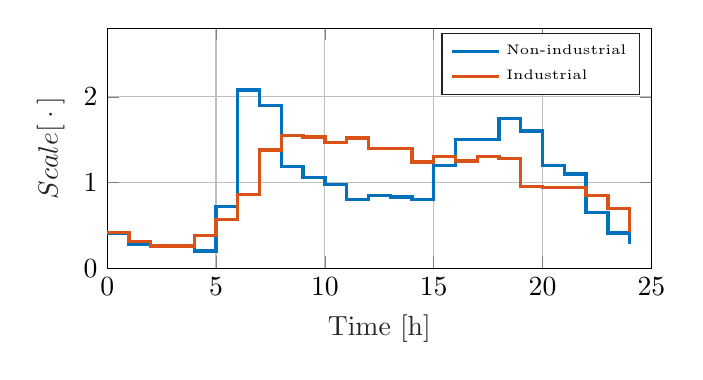
\begin{tikzpicture}

\begin{axis}[%
width=2.721in,
height=1.2in,
at={(0.758in,0.481in)},
scale only axis,
xmin=0,
xmax=25,
xlabel style={font=\color{white!15!black}},
xlabel={Time [h]},
ymin=0,
ymax=2.8,
ylabel style={font=\color{white!15!black}},
ylabel={$\text{Scale [}\cdot\text{]}$},
axis background/.style={fill=white},
%title style={font=\bfseries},
%title={Industrial/non-industrial water consumption pattern},
xmajorgrids,
ymajorgrids,
legend style={legend cell align=left, align=left, draw=white!13!black}
]
\addplot[const plot, color=mycolor1, line width=1.2pt] table[row sep=crcr] {%
0	0.41\\
1	0.280000000000001\\
2	0.25\\
3	0.260000000000002\\
4	0.199999999999999\\
5	0.719999999999999\\
6	2.08\\
7	1.9\\
8	1.19\\
9	1.06\\
10	0.98\\
11	0.800000000000001\\
12	0.850000000000001\\
13	0.829999999999998\\
14	0.800000000000001\\
15	1.2\\
16	1.5\\
18	1.75\\
19	1.6\\
20	1.2\\
21	1.1\\
22	0.649999999999999\\
23	0.41\\
24	0.280000000000001\\
};
\addlegendentry{\tiny Non-industrial}

\addplot[const plot, color=mycolor2, line width=1.2pt] table[row sep=crcr] {%
0	0.420000000000002\\
1	0.309999999999999\\
2	0.260000000000002\\
4	0.379999999999999\\
5	0.57\\
6	0.859999999999999\\
7	1.38\\
8	1.55\\
9	1.53\\
10	1.47\\
11	1.52\\
12	1.4\\
14	1.24\\
15	1.3\\
16	1.25\\
17	1.3\\
18	1.28\\
19	0.949999999999999\\
20	0.940000000000001\\
22	0.850000000000001\\
23	0.699999999999999\\
24	0.420000000000002\\
};
\addlegendentry{\tiny Industrial}

\end{axis}
\end{tikzpicture}%
\caption{Industrial and Non-industrial demand patterns implemented in EPANET.}
\label{fig:demandpatterns_EPANET}
\end{figure}

\vspace{-3mm}

In \figref{fig:demandpatterns_EPANET}, the $y$-axis shows the ratio of change compared to the base demand of the two different types of water consumption. For each type of consumer, different base demands are determined. However, the variation from this base value can be described in the same manner as the presented consumption curves for users falling in the same category. 

It is worth noting that the industrial consumption profile in the VSV zone slightly differs from the industries in the rest of the network. However, since the VSV zone is not considered in the further simulation model, the demand pattern is not shown. Furthermore, there are no individual consumers in any of the supply areas who have significant effect on the calibration and simulation of the model. 

% \subsection{Abstractions in the model}
% \label{control_and_water_source_abstractions}

% As described in \secref{the_randers_water_supply_network}, there are several different pumping stations and waterworks in the network, supplying different zones. In general, there is a possibility in EPANET to simulate the cleaning process in the waterworks, including drilling, raw water and clean water treatment. However, in the model the focus is on the correct distribution. Therefore, all waterworks are simulated with clean water reservoirs. In the EPANET simulation, pumps in the waterworks pump the water out corresponding to the real pump curves. However, there are two exceptions, where the simulation of the pumping station is different. In the OMV water work, which is responsible for filling the tanks(T1A and T1B) in HBP pumping station, the precise operation has not been taken into account. Instead, the control schedule of the pumps has been simulated as a positive demand node, which is negative according to the EPANET sign convention. The same technique was used in HBP pumping station, where the two tanks are located and which provides the distribution to the HZ. One of the reasons for this is that the controls turned out to be relatively complicated with frequency converters and the simulation result of the pumping was not matching the real world scenario. The advantage of this is that in one of the flow controlled pumping stations, the mass balance is controlled. Furthermore, the risk that the model does not simulate correctly is reduced. It should be noted that this abstraction can be done easily in HBP and OMV, since pumps in these two pumping stations are flow controlled. 

% Apart from the OMV water work and HBP pumping station, all water works have been simulated with reservoirs which cannot be emptied. Water works and pumping stations, where the pumps are pressure controlled, are controlled by PRVs, as this is the typical way of controlling pressure controlled pumps in EPANET networks \cite{agency2016epanet}. Such an arrangement is shown in \figref{fig:PRV_EPANET} 

%  %Waterworks in EPANET
% \begin{figure}[H]
% \centering
% %
\includegraphics[width=0.35\textwidth]{report/pictures/missingfigure}
% \begin{tikzpicture}[scale=0.6,transform shape]

\begin{scope} [rotate around={0:(12,5.5)}, shift={(0.8,0)}]
\draw[thick,transform shape] (12,5.5) circle (0.5);
\draw[thick,transform shape] (12.5,5.5) -- (12,6);
\draw[thick,transform shape] (12.5,5.5) node (v1) {} -- (12,5);
\end{scope}

%man-valve
\begin{scope} [rotate ={-90}]
\node(n1) at (-5.25,16) {};
\draw[thick,transform shape](n1.center) -- ($(n1)-(0.5,0)$) --
($(n1)-(0,1)$) -- ($(n1)-(0.5,1)$) --  (n1.center);

\end{scope}

\draw [thick](15,5.5) -- (13.3,5.5);
\node at (15.5,6.2) {\large PRV};
\draw [thick](16,5.5) -- (17.5,5.5);
\draw [fill=cyan] [thick](9.1,5.7) -- (9.1,5.1) -- (10.9,5.1) -- (10.9,5.7);
\draw  [thick](9.1,6.1) -- (9.1,5.1) -- (10.9,5.1) -- (10.9,6.1);
\draw [thick](12.3,5.5) -- (10.9,5.5);
\end{tikzpicture} 
% \caption{Abstraction for pressure controlled pumping stations in EPANET.}
% \label{fig:PRV_EPANET}
% \end{figure}

% \vspace{-3mm}
% It is important to note, however, that in case of high demands, with this arrangement in the network it can happen that water works and pumping stations deliver more flow than allowed or physically possible. Therefore control rules have been incorporated in the models which prevent the pumping stations produce more flow than available in the real world. 

% In case of flow controlled pumping stations, such as OMV, the following abstractions are made in the EPANET simulation framework 

%  %Flowcontrolled pumping stations in EPANET
% \begin{figure}[H]
% \centering
% %
\includegraphics[width=0.35\textwidth]{report/pictures/missingfigure}
% \begin{tikzpicture}[scale=0.65,transform shape]

\draw[fill=black] (10.7,2.2) node (v2) {} circle (.6ex);

\draw[fill=black] (11.9,2.2) node (v1) {} circle (.6ex);
\node at (12.5,3) {\large $d_+$};
\node at (14.5,3) {\large FCV};
\node at (10,3) {\large $d_-$};

\draw [-latex](v1);
\draw [thick](v1) -- (14,2.2);
\draw [thick](v2) -- (9.2,2.2);

\draw[fill=black] (9.1,2.2) node (v1) {} circle (.2ex);
\draw[fill=black] (8.7,2.2) node (v1) {} circle (.2ex);
\draw[fill=black] (8.9,2.2) node (v1) {} circle (.2ex);

\draw [-latex]  (9.4,2.7)--(10.7,2.7);
\draw [-latex](11.9,2.7) -- (13.2,2.7);

%man-valve
\begin{scope} [rotate ={-90}]
\node(n1) at (-1.95,15) {};
\draw[thick,transform shape](n1.center) -- ($(n1)-(0.5,0)$) --
($(n1)-(0,1)$) -- ($(n1)-(0.5,1)$) --  (n1.center);

\end{scope}

\draw [thick](15,2.2) -- (15.8,2.2);
\end{tikzpicture} 
% \caption{Abstraction for flow controlled pumping stations in EPANET.}
% \label{fig:FCV_EPANET}
% \end{figure}

% \vspace{-3mm}

% In \figref{fig:FCV_EPANET}, the node which has demand $d_+$ is the flow controlled pumping station. The water coming out from this node can be controlled by a FCV. In every case, the pumping stations are supplied by flow from water works. A good example for this is TBP pumping station where the water works BKV and ØSV are modelled. However, the pumping station can be modelled as two nodes, where inflow is defined on the node on the water work side and outflow is defined on the outlet side. 







